% ==============================================================
% Multi-Dimensional Apriori-Window: Exact Mining of Dense Itemset
% Regions over Arbitrary Dimensions
% ==============================================================
% Compile:
%   pdflatex main.tex && bibtex main && pdflatex main.tex && pdflatex main.tex
% ==============================================================
\documentclass[conference]{IEEEtran}
\IEEEoverridecommandlockouts

% --- Standard packages ---
\usepackage{cite}
\usepackage{amsmath,amssymb,amsfonts}
\usepackage{amsthm}
\usepackage{algorithm}
\usepackage{algpseudocode}
\usepackage{graphicx}
\usepackage{textcomp}
\usepackage{xcolor}
\usepackage{threeparttable}
\usepackage{subcaption}
\usepackage{booktabs}
\usepackage{url}
\usepackage{multirow}
\usepackage{bm}
\usepackage{tikz}
\usetikzlibrary{arrows.meta, positioning, shapes.geometric, fit}

% --- Theorem environments ---
\newtheorem{definition}{Definition}
\newtheorem{theorem}{Theorem}
\newtheorem{lemma}{Lemma}
\newtheorem{remark}{Remark}
\newtheorem{example}{Example}

\def\BibTeX{{\rm B\kern-.05em{\sc i\kern-.025em b}\kern-.08em
    T\kern-.1667em\lower.7ex\hbox{E}\kern-.125emX}}

\begin{document}
\bstctlcite{IEEEexample:BSTcontrol}

\title{Multi-Dimensional Apriori-Window: \\
Exact Mining of Dense Itemset Regions\\
over Arbitrary Dimensions}

\author{
  \IEEEauthorblockN{Kanata Takayasu}
  \IEEEauthorblockA{
    \textit{Keio University}\\
    Yokohama, Japan\\
    kanata1222@keio.jp}
  \and
  \IEEEauthorblockN{Taihei Takahashi}
  \IEEEauthorblockA{
    \textit{Keio University}\\
    Yokohama, Japan\\
    taihei-t@keio.jp}
  \and
  \IEEEauthorblockN{Satoshi Suga}
  \IEEEauthorblockA{
    \textit{Kansai University}\\
    Osaka, Japan\\
    stssg526@gmail.com}
  \and
  \IEEEauthorblockN{Satoshi Kurihara}
  \IEEEauthorblockA{
    \textit{Keio University}\\
    Yokohama, Japan\\
    satoshi@keio.jp}
}

\maketitle
\pagestyle{empty}

\begin{abstract}
In large-scale retail, epidemiology, and logistics data,
analysts need to determine both
\emph{what} is dense (itemsets) and
\emph{when and where} it is dense (spatio-temporal regions)
simultaneously.
However, existing methods cannot achieve both:
pattern mining methods do not output regions,
while region extraction methods (e.g., M-Zoom)
cannot be integrated with itemset enumeration
due to their Cartesian-product block constraints
and lack of anti-monotonicity.
This paper proposes \textbf{Multi-Dimensional Apriori-Window},
which exactly extracts all dense itemsets together with
their dense regions over arbitrary $d$-dimensional grids.
By reducing the multi-dimensional problem
to a duplicate-aware one-dimensional problem
for each fixed spatial start point,
and by exploiting the anti-monotonicity
of windowed support counts for Apriori pruning,
the method exactly enumerates all dense patterns
together with their arbitrarily-shaped dense regions.

The proposed method also exactly extracts all dense patterns
and their dense regions by construction
(F1 $= 1.00$, Jaccard $= 1.00$).
Comparative experiments on synthetic data
with diverse embedded dense-region shapes
show that pattern mining baselines achieve
a pattern detection F1 of only 0.356--0.917,
with substantial variation depending on the region shape.
Region extraction baselines (MZoom, LISA, ST-DBSCAN),
even when given ground truth patterns,
achieve mean Jaccard $\leq$ 0.190,
failing to closely approximate the sliding-window dense regions.
In contrast, scalability experiments reveal
the proposed method achieves linear scaling
over four orders of magnitude
($N = 10^4$--$10^8$ transactions),
processing $10^8$ transactions within 9 minutes.
When applied to $d{=}3$--$4$ real-world data from crime,
complaints, and earthquake domains,
the method yields interpretable insights
consistent with domain knowledge.
\end{abstract}

\begin{IEEEkeywords}
Frequent pattern mining, multi-dimensional data, sliding window,
dense region detection, Apriori, interval representation
\end{IEEEkeywords}

% ==============================================================
\section{Introduction}\label{sec:intro}
% ==============================================================

\subsection{Motivation and Application Background}

Data analysts at large retail chains want to know
``which product combinations are intensively purchased,
at which store locations, and during which time periods.''
For example, from 100 stores $\times$ 52 weeks of
point-of-sale data, the insight that
``sales of beer and potato chips are concentrated during
weeks 46--52 (year-end season) at urban stores (stores 0--9)''
directly informs region-specific inventory planning
and promotional strategies.
Similarly, in epidemiology, specific regions and periods
in which co-occurrence patterns of symptoms are concentrated
become intervention targets.
In logistics, regional and temporal surges in shipment volumes
support service optimization.

Multi-dimensional data are thus accumulated across many domains,
and extracting \emph{spatio-temporally localized dense patterns}
from such data can contribute to discovering knowledge
beyond that provided by conventional aggregate analysis.

\subsection{Limitations of Existing Methods}

In the above applications, analysts truly need to know two things:
(i)~\emph{what} is dense (itemset $P$) and
(ii)~\emph{when and where} it is dense ($d$-dimensional dense region),
i.e., the tuple $(P, R(P))$.
Pattern $P$ alone leaves ``which store to reorder to and when'' unknown,
while region $R$ alone leaves ``what to reorder'' unspecified.
Only when both are available can region- and period-specific
strategies be formulated.
However, no existing method provides both simultaneously.

\paragraph{Pattern mining methods.}
Frequent pattern mining~\cite{agrawal1994apriori,han2000mining}
relies on global support and thus misses locally dense patterns.
Existing methods that consider locality~\cite{aprioriwindow}
remain limited to a one-dimensional design on the temporal axis
and cannot exploit multi-dimensional spatial information.
\paragraph{Region extraction methods.}
Dense subtensor mining (M-Zoom~\cite{shin2016mzoom}, etc.)
cannot fit arbitrarily-shaped dense regions
due to Cartesian-product block constraints,
and it inaccurately enumerates patterns
(detailed in \S\ref{sec:related}).
Spatial statistics methods~\cite{anselin1995lisa,ord1995getis}
cannot handle the temporal dimension.
Scan statistics~\cite{kulldorff1997spatial}
lack the concept of itemsets.
ST-DBSCAN~\cite{birant2007stdbscan} relies on
point-neighborhood density and thus cannot detect
localized concentrations distinguished from background density;
it also lacks anti-monotonicity and therefore
cannot be integrated with Apriori pruning.

\subsection{Contributions of This Work}

This paper proposes
\textbf{Multi-Dimensional Apriori-Window},
which exactly extracts all dense patterns and their dense regions
over arbitrary $d$-dimensional grids
(time + $d{-}1$ spatial/categorical dimensions)
(\S\ref{sec:method}).
In a nutshell, the proposed method enables analysts to
\textbf{exactly extract ``what sells when and where''
under the sliding-window density definition}.

The technical essence of this work lies in extending
the dense interval computation of
one-dimensional Apriori-Window~\cite{aprioriwindow}
to $d$ dimensions by applying it to
the temporal multiset for each fixed spatial start point.
That is, even after multi-dimensionalization,
the core computation is essentially
a \emph{duplicate-aware one-dimensional Apriori-Window}.

Three techniques realize this multi-dimensionalization.

\begin{enumerate}
\item \textbf{Reduction to 1D per fixed spatial start point}:
For each spatial start point $\bm{s}_{\mathrm{sp}}$,
occurrences of a pattern falling into the spatial window
are collapsed into a temporal multiset
$L_P(\bm{s}_{\mathrm{sp}})$.
This decomposes the $d$-dimensional problem
into multiple one-dimensional problems
keyed by spatial start points.

\item \textbf{Apriori pruning via $(k{-}1)$-subset interval map intersection}:
Dense regions from the previous level are maintained
as temporal interval sequences per spatial start point.
For candidate patterns, these are intersected
to form candidate intervals.
This enables interval-based pruning
isomorphic to the 1D case for $k \geq 2$
(Lemma~\ref{lem:apriori}).

\item \textbf{Duplicate-aware $t$-axis stride}:
In two or more dimensions, duplicate timestamps arise.
Instead of maintaining dense-start positions one by one,
contiguous blocks of left endpoints guaranteed to be dense
by the current window alone are processed in bulk,
and output as dense intervals (Lemma~\ref{lem:stride}).
\end{enumerate}

% ==============================================================
\section{Related Work}\label{sec:related}
% ==============================================================

This work addresses the problem of discovering
dense itemset regions from spatio-temporal transaction data.
This problem lies at the intersection of two research lineages:
(1)~the \emph{pattern mining lineage} aimed at enumerating itemsets, and
(2)~the \emph{dense block detection lineage} aimed at detecting
dense blocks in multi-dimensional spaces.
Below we organize both lineages and clarify
why this work is positioned at their intersection.

% ==============================================================
\subsection{Pattern Mining Lineage}
% ==============================================================

\paragraph{Frequent Itemset Mining (FIM).}
The Apriori algorithm by Agrawal et al.~\cite{agrawal1994apriori}
exploits the monotonicity of itemsets
(subsets always have no less support than their supersets)
to drastically prune the candidate space.
FP-Growth by Han et al.~\cite{han2000mining}
further accelerates mining using prefix trees.
These methods use global support over the entire
static transaction database as their criterion,
and thus suffer from the fundamental problem
of missing locally dense patterns~\cite{aprioriwindow}.

\paragraph{Local dense interval detection methods.}
Several methods based on \emph{intervals} between consecutive
occurrence timestamps have been proposed
for detecting locally dense intervals.
LPFIM~\cite{mahanta2005lpfim} splits intervals
when the gap between two consecutive occurrences exceeds
a threshold minthd1, and outputs intervals
whose local support rate exceeds a threshold
and whose length exceeds minthd2.
LPPM~\cite{fournierviger2021lppm} introduces
spillover accumulation for noise-robust interval detection.

These methods estimate density by evaluating
``the time difference between two consecutive occurrences
(inter-occurrence interval).''
However, as pointed out in~\cite{aprioriwindow},
since the gap parameter governs both pattern identification accuracy
and interval detection accuracy,
parameter settings that simultaneously keep both high
generally do not exist.
Moreover, these methods are \emph{inherently non-extensible to
multiple dimensions}.
Occurrence points on a $d$-dimensional grid
have no linear ordering,
making ``the interval between two consecutive occurrences''
ill-defined.

Apriori-Window~\cite{aprioriwindow} is an exact method
that resolves this structural limitation.
By \emph{directly} computing the number of occurrences
within a sliding window $[l, l+W]$
rather than via inter-occurrence intervals,
it evaluates local frequency without requiring a gap parameter.
Combined with anti-monotonicity-based Apriori pruning
and $t$-axis stride, it exhaustively and exactly
enumerates dense intervals.
Comparative experiments demonstrated that
Apriori-Window significantly outperforms
LPFIM and LPPM~\cite{aprioriwindow}.

\emph{Why multi-dimensionalization is possible}:
The definition ``number of occurrences within a rectangular window''
naturally extends to $d$ dimensions
(simply replacing the window with a $d$-dimensional hyperrectangle
$\prod_k [s_k, s_k+W_k]$).
In contrast to interval-based methods
that depend on linear ordering,
the design of Apriori-Window does not require linear ordering.
This work builds on this observation to extend
Apriori-Window from one dimension to arbitrary $d$ dimensions.

\paragraph{Colocation mining.}
Colocation mining~\cite{shekhar2001colocation}
evaluates patterns where multiple feature types
co-exist in geographic proximity
using the Participation Index (PI).
Qian et al.~\cite{qian2009stcolocation} extended this
to weighted sliding windows (STCP-Miner).
These methods deal with spatial proximity-based co-occurrence
rather than transaction-based co-occurrence
and do not extract dense regions.
However, they can be compared in terms of
pattern identification accuracy (F1) (\S\ref{sec:ex1_1}).

% ==============================================================
\subsection{Region Extraction Lineage}
% ==============================================================

% --- Dense block detection ---
\paragraph{Dense block detection methods.}
Dense block detection methods
including M-Zoom~\cite{shin2016mzoom}
and others (tensor:~\cite{jiang2015crossspot,shin2018mbiz,shin2017dcube,shin2017densealert,feng2020catchcore};
graph: SpecGreedy~\cite{feng2020specgreedy})
detect dense blocks in multi-dimensional data.
They select value sets $B_k \subseteq D_k$ along each dimension
and perform greedy search to maximize
the mass-to-volume ratio of the Cartesian-product block
$\prod_k B_k$.

These methods have two structural limitations.

\emph{First, output is restricted to Cartesian-product blocks.}
For irregularly-shaped dense regions,
they inevitably include excessive areas
or miss dense cells,
resulting in low Jaccard even when GT patterns are provided
(demonstrated in \S\ref{sec:ex1_1}).

\emph{Second, pattern enumeration is inaccurate.}
While adding items as an additional dimension
allows enumeration to be attempted,
the Cartesian-product constraint causes all subsets
of the itemset $C_B$ within a block
to be assumed dense in the same region,
generating false positives (demonstrated in \S\ref{sec:ex1_1}).

% --- Spatial statistics ---
\paragraph{Spatial statistics.}
LISA~\cite{anselin1995lisa} identifies spatial hotspots
using local Moran's $I$, and
Getis-Ord $G_i^*$~\cite{ord1995getis} evaluates
local concentration via $z$-scores.
Both target \emph{spatial dimensions only};
running them per time slice
loses temporal continuity.

% --- Spatial/spatio-temporal scan statistics ---
\paragraph{Spatial and spatio-temporal scan statistics.}
Kulldorff's~\cite{kulldorff1997spatial,kulldorff2001prospective}
spatial/spatio-temporal scan statistics detect
significant clusters using circular/cylindrical scanning windows.
FlexScan~\cite{tango2005flexscan} extends this
to irregularly-shaped windows.

All above statistical methods are designed
to detect per-variable anomalous concentrations
and cannot enumerate co-occurrence patterns (itemsets)
within transactions.
Enumerating all patterns would require
$O(2^{|\mathcal{I}|})$ independent runs,
and integration with Apriori pruning is not part of their design.

% --- Spatio-temporal clustering ---
\paragraph{Spatio-temporal density-based clustering (ST-DBSCAN, etc.).}
ST-DBSCAN~\cite{birant2007stdbscan} extends
DBSCAN~\cite{ester1996dbscan} to spatio-temporal data
with independent thresholds $\varepsilon_1, \varepsilon_2$
for spatial and temporal distances.
While it outputs arbitrarily-shaped clusters,
first, it defines density by point-neighborhood counts;
when occurrences are spatially uniform,
the entire dataset becomes a single cluster,
failing to identify localized concentrations.
Second, point-neighborhood density lacks anti-monotonicity,
making independent processing of all patterns
$O(2^{|\mathcal{I}|})$ unavoidable.

All above region extraction methods lack the concept of itemsets,
but they can be evaluated as region extractors
when GT patterns and their occurrence densities are provided
(\S\ref{sec:ex1_1}).

% ==============================================================
\subsection{Positioning of This Work}
% ==============================================================

The above analysis shows that no existing method
simultaneously enumerates patterns
and extracts multi-dimensional dense regions.
This work achieves both within a single framework
by exploiting the anti-monotonicity
of windowed-occurrence-based density
to naturally integrate Apriori pruning.
Table~\ref{tab:related} illustrates this positioning.

\paragraph{Why no stronger baseline exists.}
The gap in Table~\ref{tab:related} reflects a \emph{structural} incompatibility:
pattern mining methods cannot output spatio-temporal windows,
and region extraction methods lose Apriori pruning when applied independently per itemset.
Faster variants within the same categories share these limitations;
the chosen baselines therefore represent each distinct methodological category.

\begin{table}[t]
\centering
\caption{Comparison with related methods.
``Itemset'' refers to the ability to enumerate patterns;
``Dense region'' refers to the ability to output
spatio-temporally localized dense regions.}
\label{tab:related}
\small
\begin{tabular}{lccc}
\toprule
Method & \shortstack{Item-\\set} & \shortstack{ST dense\\region} & \shortstack{Region\\shape} \\
\midrule
Apriori~\cite{agrawal1994apriori}
                                          & $\checkmark$ & $\times$     & ---          \\
LPFIM~\cite{mahanta2005lpfim} et al.
                                          & $\checkmark$ & 1D only      & Interval     \\
Apriori-Window~\cite{aprioriwindow}       & $\checkmark$ & 1D only      & Interval     \\
Colocation~\cite{shekhar2001colocation}
                                          & $\checkmark$ & $\times$     & ---          \\
STCP-Miner~\cite{qian2009stcolocation}   & $\checkmark$ & $\times$     & ---          \\
\midrule
M-Zoom~\cite{shin2016mzoom} et al.       & $\triangle$$^*$     & $\checkmark$ & Cartesian only \\
SaTScan~\cite{kulldorff1997spatial}       & $\times$     & $\checkmark$ & Circle/cylinder \\
FlexScan~\cite{tango2005flexscan}        & $\times$     & $\checkmark$ & Irregular    \\
LISA~\cite{anselin1995lisa}
  / $G_i^*$~\cite{ord1995getis}          & $\times$     & Spatial only & Arbitrary    \\
ST-DBSCAN~\cite{birant2007stdbscan} et al. & $\times$   & $\checkmark$ & Arbitrary    \\
\midrule
\textbf{Ours}                              & $\checkmark$ & $\checkmark$ & Arbitrary    \\
\bottomrule
\multicolumn{4}{l}{\scriptsize $^*$Patterns can be output by including items as a dimension,} \\
\multicolumn{4}{l}{\scriptsize \hspace{1em}but Cartesian constraints cause false positives and preclude region separation.}
\end{tabular}
\end{table}

% ==============================================================
\section{Problem Definition}\label{sec:problem}
% ==============================================================

This section reviews the one-dimensional setting
of Apriori-Window~\cite{aprioriwindow} (\S\ref{sec:1d_review})
and then formulates its $d$-dimensional extension (\S\ref{sec:nd_extension}).

% ==============================================================
\subsection{Apriori-Window (One-Dimensional)}\label{sec:1d_review}
% ==============================================================

Let $\mathcal{I} = \{i_1, \ldots, i_m\}$ be the item universe and
$\mathcal{D}_{\mathrm{1D}} = \{(t_n, d_n)\}_{n=1}^N$
be a timestamped transaction sequence,
where $t_n \in \mathbb{Z}_{\geq 0}$ is an integer timestamp
and $d_n \subseteq \mathcal{I}$ is an itemset.

The occurrence sequence of a pattern $P \subseteq \mathcal{I}$ is
\[
  \mathrm{occ}(P) = \{t_n : P \subseteq d_n\}.
\]

\begin{definition}[Interval support~\cite{aprioriwindow}]\label{def:sup1d}
Under window width $W$ ($W > 0$),
the interval support of pattern $P$
at window left endpoint $l$ is defined as
\[
  \mathrm{sup}(P,\, l,\, W)
  = \bigl|\{t \in \mathrm{occ}(P) : l \leq t \leq l + W\}\bigr|.
\]
The window $[l, l+W]$ contains $W+1$ discrete time points.
\end{definition}

\begin{definition}[Dense-start set and dense interval]\label{def:dense1d}
For a support threshold $\theta$,
\[
  \mathcal{T}_\theta(P)
  = \{l \in \mathbb{Z}_{\geq 0} : \mathrm{sup}(P, l, W) \geq \theta\}
\]
is the \emph{dense-start set} of $P$.

Let $[a,b] \subseteq \mathcal{T}_\theta(P)$
be a maximal contiguous component.
Then $[a,\, b + W]$ is called a \emph{dense interval} of $P$.
\end{definition}


% ==============================================================
\subsection{Extension to $d$ Dimensions}\label{sec:nd_extension}
% ==============================================================

Let $\mathcal{D} = \{(\bm{b}_n, d_n)\}_{n=1}^N$
be a $d$-dimensional transaction sequence, where
\[
  \bm{b}_n = (b_n^{(0)}, b_n^{(1)}, \ldots, b_n^{(d-1)})
  \in \prod_{k=0}^{d-1}\{0,1,\ldots,N_k-1\}
\]
is an integer coordinate vector (axis 0 is time) and
$d_n \subseteq \mathcal{I}$ is an itemset.
$N$ denotes the \emph{number of transactions}.

\begin{definition}[Temporal multiset reduction to a fixed spatial start point]\label{def:collapsed_multiset_nd}
Fix a spatial start vector
\[
  \bm{s}_{\mathrm{sp}} = (s_1, \ldots, s_{d-1})
\]
and spatial window widths
$\bm{W}_{\mathrm{sp}} = (W_1, \ldots, W_{d-1})$
(each $W_k > 0$).
The spatial window along axis $k$, $[s_k, s_k + W_k]$,
contains $W_k + 1$ discrete coordinates.
The temporal multiset of pattern $P$ is defined as
\[
  L_P(\bm{s}_{\mathrm{sp}})
  =
  \{\!\{
    b_n^{(0)}
    \mid
    P \subseteq d_n,\;
    s_k \leq b_n^{(k)} \leq s_k + W_k\; (\forall k=1,\ldots,d-1)
  \}\!\}
\]
where $\{\!\{\cdot\}\!\}$ denotes a multiset allowing duplicates.
\end{definition}

The essence of this definition is that,
for each fixed spatial start point,
the $d$-dimensional problem is reduced to
a \emph{one-dimensional problem with duplicate timestamps}.

\begin{definition}[$d$-dimensional sliding window support]\label{def:support_nd}
For a temporal start point $s_0$ and spatial start vector
$\bm{s}_{\mathrm{sp}}$,
the support of pattern $P$ is defined as
\begin{equation}\label{eq:support_nd}
  S_P(s_0, \bm{s}_{\mathrm{sp}})
  = \bigl|\{t \in L_P(\bm{s}_{\mathrm{sp}}) : s_0 \leq t \leq s_0 + W_0\}\bigr|.
\end{equation}
\end{definition}

\begin{definition}[Dense-start set and dense region]\label{def:dense_region_nd}
For a fixed spatial start vector $\bm{s}_{\mathrm{sp}}$,
\[
  \mathcal{T}_\theta(P,\bm{s}_{\mathrm{sp}})
  =
  \{s_0 \in \mathbb{Z}_{\geq 0} : S_P(s_0,\bm{s}_{\mathrm{sp}}) \geq \theta\}
\]
is the \emph{dense-start set} of $P$
at $\bm{s}_{\mathrm{sp}}$.

Let $[a_j,b_j]$ be a maximal contiguous component
of $\mathcal{T}_\theta(P,\bm{s}_{\mathrm{sp}})$.
Then $[a_j,\, b_j + W_0]$ is called a \emph{dense interval} of $P$
at $\bm{s}_{\mathrm{sp}}$
(a natural extension of Definition~\ref{def:dense1d}).

The collection of dense intervals over all spatial start points,
\[
  \mathcal{R}_\theta(P)
  = \{(\bm{s}_{\mathrm{sp}},\, [a_j,\, b_j + W_0])\},
\]
is called the \emph{dense region} of $P$.
\end{definition}

\paragraph{Apriori monotonicity.}

\begin{lemma}[Monotonicity of dense-start sets]\label{lem:apriori}
For any pattern $P$ and its subset $Q \subset P$,
and any spatial start vector $\bm{s}_{\mathrm{sp}}$,
\[
  \mathcal{T}_\theta(P,\bm{s}_{\mathrm{sp}})
  \subseteq
  \mathcal{T}_\theta(Q,\bm{s}_{\mathrm{sp}})
\]
holds.
\end{lemma}

The proof is given in Appendix~\ref{sec:proofs}.

By Lemma~\ref{lem:apriori},
the dense-start set of a size-$k$ pattern $P$
is contained within the dense intervals
of each $(k{-}1)$-subset of $P$.
The proposed method exploits this property
by using \emph{intersection of $(k{-}1)$-subset interval maps}
as candidate intervals (\S\ref{sec:alg_k2}).

\subsection{$d$-Dimensional Dense Region Detection Problem}\label{sec:dense_detection}

The $d$-dimensional dense region detection problem is
(given a $d$-dimensional transaction sequence $\mathcal{D}$,
window widths
$\bm{W} = (W_0, W_1, \ldots, W_{d-1}) \in \mathbb{Z}_{>0}^d$,
and a support threshold $\theta$)
to find the complete set of dense regions
$\mathcal{R}_\theta(P)
= \{(\bm{s}_{\mathrm{sp}}, [a_j,\, b_j + W_0])\}$
for each pattern $P$.
The window along each axis $k$ is a closed interval
$[s_k, s_k + W_k]$ ($W_k + 1$ bins).

% ==============================================================
\section{Proposed Method: Multi-Dimensional Apriori-Window Algorithm}
\label{sec:method}
% ==============================================================

We propose the \textbf{Multi-Dimensional Apriori-Window algorithm}
to solve the problem in \S\ref{sec:dense_detection}.

% ==============================================================
\subsection{1D Multiset Reduction via Fixed Spatial Start Points}\label{sec:binsearch}
% ==============================================================

For a pattern $P$ and a fixed spatial start point
$\bm{s}_{\mathrm{sp}}$,
we construct the temporal multiset
$L_P(\bm{s}_{\mathrm{sp}})$
from Definition~\ref{def:collapsed_multiset_nd}.
This is obtained by distributing each occurrence transaction of $P$
to all spatial start points whose window contains that transaction.

\paragraph{Distribution to spatial start points.}
When a transaction containing pattern $P$
resides at discrete coordinates
\[
  \bm{b} = (b^{(0)}, b^{(1)}, \ldots, b^{(d-1)}),
\]
the $k$-th component ($k \geq 1$)
of a spatial start point containing this transaction satisfies
\[
  s_k \in [\max(0,\, b^{(k)} - W_k),\; b^{(k)}].
\]
Therefore, one occurrence contributes to at most
\[
  W_{\mathrm{sp}} = \prod_{k=1}^{d-1} (W_k + 1)
\]
spatial start points.

\paragraph{Construction cost.}
Let $N_P$ denote the number of occurrence transactions of pattern $P$.
Construction costs $O(N_P \cdot W_{\mathrm{sp}})$;
including sorting, the total is $O(\widetilde N_P \log \widetilde N_P)$
where $\widetilde N_P = N_P \cdot W_{\mathrm{sp}}$.

% ==============================================================
\subsection{Duplicate-Aware Interval Solver on the $t$-Axis}\label{sec:t_stride}
% ==============================================================

For a fixed spatial start point $\bm{s}_{\mathrm{sp}}$,
we compute dense intervals from the sorted multiset
$L = L_P(\bm{s}_{\mathrm{sp}})$.
In two or more dimensions,
multiple transactions may share the same timestamp,
producing duplicates in $L$.
Consequently, the 1D Apriori-Window algorithm~\cite{aprioriwindow}
cannot be applied to this multiset straightforwardly.

The key idea is a two-branch stride
governed by the comparison of
the window count $c$ and the threshold $\theta$
(Figure~\ref{fig:t_stride}).
When $c < \theta$ (non-dense),
the left endpoint $l$ jumps to the position
where the next event enters the window,
skipping unnecessary scans
(Eq.~\eqref{eq:jump_empty}, Figure~\ref{fig:t_stride}(b)).
When $c \geq \theta$ (dense),
the surplus $c - \theta$ determines
a contiguous block $[l, l_{\mathrm{dense}}]$ of left endpoints
that are all guaranteed to be dense,
and this entire block is output as a dense interval in bulk
(Eq.~\eqref{eq:jump_dense}, Figure~\ref{fig:t_stride}(a)).
The correctness of this bulk processing
is guaranteed by Lemma~\ref{lem:stride}.

Specifically, the left endpoint update in the non-dense case is
\begin{equation}\label{eq:jump_empty}
  l \leftarrow \max(l+1,\; L[\mathrm{next}] - W_0)
\end{equation}
where $L[\mathrm{next}]$ is the first event
outside the right boundary of the current window.
In the dense case, the block right boundary is
\begin{equation}\label{eq:jump_dense}
  l_{\mathrm{dense}} = L[l_{\mathrm{lo}} + (c - \theta)]
\end{equation}
where $l_{\mathrm{lo}}$ is the first position in $L$
that is $\geq l$.
The dense interval's right endpoint is extended to
$l_{\mathrm{dense}} + W_0$,
and the left endpoint is updated to
$l \leftarrow l_{\mathrm{dense}} + 1$.

\begin{lemma}[Correctness of the dense block]\label{lem:stride}
For $l_{\mathrm{dense}}$ defined by Eq.~\eqref{eq:jump_dense},
for any $l' \in [l,\, l_{\mathrm{dense}}]$,
\[
  |\{t \in L : l' \leq t \leq l' + W_0\}| \geq \theta
\]
holds.
\end{lemma}

The proof is given in Appendix~\ref{sec:proofs}.

\begin{figure}[t]
\centering
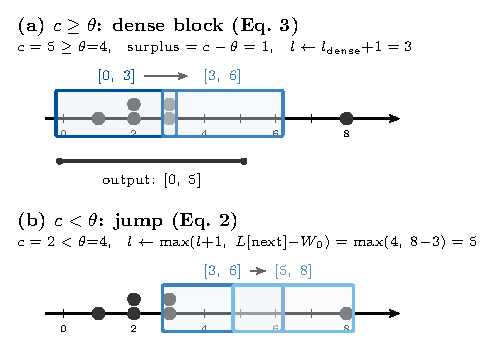
\includegraphics[width=0.75\columnwidth]{fig/fig3_t_stride.pdf}
\caption{Duplicate-aware $t$-axis stride.
Given a sorted multiset
$L = \{\!\{1, 2, 2, 3, 3, 8\}\!\}$
with $W_0{=}3$ and $\theta{=}4$.
(a)~When $c \geq \theta$,
the surplus determines how far the left endpoint
can stride in bulk (Eq.~\eqref{eq:jump_dense}).
(b)~When $c < \theta$,
the window jumps to the next position
where a new event enters (Eq.~\eqref{eq:jump_empty}).
Window color gradient (dark$\to$light blue)
indicates the progression of the left endpoint $l$.}
\label{fig:t_stride}
\end{figure}

\begin{algorithm}[t]
\caption{Duplicate-aware dense interval computation for a fixed spatial start point}
\label{alg:t_stride}
\begin{algorithmic}[1]
\Require Sorted multiset $L$, temporal window width $W_0$, threshold $\theta$
\Ensure Dense interval sequence $\mathcal{R}$
\State $\mathcal{R} \leftarrow \emptyset$
\State $l \leftarrow \max(0,\, L[\theta-1] - W_0)$
\State $\mathit{open} \leftarrow \mathrm{false}$
\While{$l \leq L[\mathrm{last}]$}
  \State $l_{\mathrm{lo}} \leftarrow \mathrm{lower\_bound}(L, l)$
  \State $l_{\mathrm{hi}} \leftarrow \mathrm{upper\_bound}(L, l + W_0)$
  \State $c \leftarrow l_{\mathrm{hi}} - l_{\mathrm{lo}}$
  \If{$c < \theta$}
    \If{$\mathit{open}$}
      \State Append current interval to $\mathcal{R}$
      \State $\mathit{open} \leftarrow \mathrm{false}$
    \EndIf
    \If{$l_{\mathrm{hi}} = |L|$} \textbf{break} \EndIf
    \State $l \leftarrow \max(l+1,\; L[l_{\mathrm{hi}}] - W_0)$
           \Comment{Eq.~\eqref{eq:jump_empty}}
  \Else
    \State $l_{\mathrm{dense}} \leftarrow L[l_{\mathrm{lo}} + (c-\theta)]$
           \Comment{Eq.~\eqref{eq:jump_dense}}
    \State $r_{\mathrm{block}} \leftarrow l_{\mathrm{dense}} + W_0$
    \State Start or extend current interval with $(l, r_{\mathrm{block}})$
    \State $\mathit{open} \leftarrow \mathrm{true}$
    \State $l \leftarrow l_{\mathrm{dense}} + 1$
  \EndIf
\EndWhile
\If{$\mathit{open}$}
  \State Append current interval to $\mathcal{R}$
\EndIf
\State \Return $\mathcal{R}$
\end{algorithmic}
\end{algorithm}

% ==============================================================
\subsection{Candidate Interval Restriction via Apriori Pruning ($k \geq 2$)}\label{sec:alg_k2}
% ==============================================================

By applying Lemma~\ref{lem:apriori} recursively,
any dense-start component of a size-$k$ pattern $P$
is contained within the dense intervals
of each $(k{-}1)$-subset of $P$.
Using this property,
we use \emph{intersections of $(k{-}1)$-subset interval maps}
for candidate patterns $P$.

\paragraph{Candidate interval map.}
Let the dense region of pattern $Q$ be
\[
  \mathcal{R}_\theta(Q)
  = \{(\bm{s}_{\mathrm{sp}}, [a,e])\}.
\]
Write $\mathcal{R}_\theta(Q)[\bm{s}_{\mathrm{sp}}]$
for the temporal interval sequence
belonging to the same spatial start point $\bm{s}_{\mathrm{sp}}$.
The candidate interval map for a size-$k$ pattern $P$ is then defined as
\begin{equation}\label{eq:candidate_cells}
  \mathcal{C}(P,\bm{s}_{\mathrm{sp}})
  =
  \bigcap_{Q \in \binom{P}{k-1}}
  \mathcal{R}_\theta(Q)[\bm{s}_{\mathrm{sp}}].
\end{equation}

Here the intersection is the standard interval intersection
on temporal intervals, and $\binom{P}{k-1}$ is the set of all
$(k{-}1)$-subsets of $P$.
If $\mathcal{C}(P,\bm{s}_{\mathrm{sp}})=\emptyset$
for all spatial start points,
$P$ cannot have any dense interval and is pruned.
For $k=2$, $\binom{P}{1}$ reduces to singletons,
so this is a generalization of the singleton intersection.

\paragraph{Exact re-evaluation.}
Only when $\mathcal{C}(P,\bm{s}_{\mathrm{sp}}) \neq \emptyset$,
we scan the transaction sequence once
to construct $L_P(\bm{s}_{\mathrm{sp}})$
and run the candidate-interval version of
Algorithm~\ref{alg:t_stride}
over $\mathcal{C}(P,\bm{s}_{\mathrm{sp}})$.

% ==============================================================
\subsection{Overall Algorithm and Complexity}\label{sec:complexity}
% ==============================================================

\begin{algorithm}[t]
\caption{Multi-Dimensional Apriori-Window (interval-based implementation)}
\label{alg:md_apriori}
\begin{algorithmic}[1]
\Require $d$-dimensional transaction sequence $\mathcal{D}$, $(\bm{W}, \theta)$
\Ensure Dense region $\mathcal{R}_\theta(P)$ for each pattern $P$
\ForAll{$i \in \mathcal{I}$}
  \State $L_i(\bm{s}_{\mathrm{sp}}) \leftarrow$ Construct temporal multiset per spatial start point
  \State $\mathcal{R}_\theta(\{i\}) \leftarrow$ Run Algorithm~\ref{alg:t_stride} for each $\bm{s}_{\mathrm{sp}}$
\EndFor
\State $\mathcal{F}_1 \leftarrow \{\{i\} : \mathcal{R}_\theta(\{i\}) \neq \emptyset\}$
\State $k \leftarrow 2$
\While{$\mathcal{F}_{k-1} \neq \emptyset$}
  \State \texttt{cands} $\leftarrow$ \Call{GenerateCandidates}{$\mathcal{F}_{k-1}$}
  \State \texttt{cands} $\leftarrow$ \Call{PruneCandidates}{\texttt{cands}, $\mathcal{F}_{k-1}$}
  \State $\mathcal{F}_k \leftarrow \emptyset$
  \ForAll{$P \in$ \texttt{cands}}
    \State $\mathcal{C}(P,\bm{s}_{\mathrm{sp}}) \leftarrow \bigcap_{Q \in \binom{P}{k-1}}\mathcal{R}_\theta(Q)[\bm{s}_{\mathrm{sp}}]$
           \Comment{Eq.~\eqref{eq:candidate_cells}}
    \If{$\mathcal{C}(P,\bm{s}_{\mathrm{sp}})=\emptyset$ for all $\bm{s}_{\mathrm{sp}}$}
      \State \textbf{continue}
    \EndIf
    \State $L_P(\bm{s}_{\mathrm{sp}}) \leftarrow$ Construct temporal multiset for pattern $P$
    \State $\mathcal{R}_\theta(P) \leftarrow$ Run candidate-interval duplicate-aware solver for each $\bm{s}_{\mathrm{sp}}$
    \If{$\mathcal{R}_\theta(P) \neq \emptyset$}
      \State $\mathcal{F}_k \leftarrow \mathcal{F}_k \cup \{P\}$
    \EndIf
  \EndFor
  \State $k \leftarrow k + 1$
\EndWhile
\State \Return $\{\mathcal{R}_\theta(P)\}$
\end{algorithmic}
\end{algorithm}

Per-step complexity breakdown and the overall complexity formula
are given in Appendix~\ref{sec:complexity_appendix}.
When applied to real data,
continuous coordinates need to be discretized
as a preprocessing step (\S\ref{sec:experiments}).

% ==============================================================
\section{Experiments}\label{sec:experiments}
% ==============================================================

We verified the scalability and effectiveness of the proposed method.
All experiments were implemented in Rust (release build)
and executed on Apple M3 (8 cores, 24\,GB RAM).

% ==============================================================
\subsection{EX-1: Exactness Verification on Synthetic Data}
\label{sec:ex1}\label{sec:ex1_1}
% ==============================================================

\paragraph{Objective.}
Synthetic data with four embedding shapes
(rectangular, drift, intermittent, and expanding)
was used to verify how well existing methods recover
the exact solution defined by the proposed method.

\paragraph{Synthetic data.}
A grid with $T{=}100$ temporal and $S{=}100$ spatial grid points containing 20 embedded GT patterns,
with 3 seeds per shape ($4 \times 3 = 12$ datasets in total).
Generation details are given in Appendix~\ref{sec:ex1_data_details}.

\paragraph{Baseline methods.}
Each baseline addresses a fundamentally different formulation,
so all tunable parameters were grid-searched to maximize each baseline's score for a fair comparison.
Colocation / STCP-Miner are used in EX-1-1 (pattern detection);
LISA / MZoom / ST-DBSCAN are used in EX-1-2 (region recovery).

\begin{itemize}
\item \textbf{Colocation}~\cite{shekhar2001colocation}: Spatial colocation mining. PI threshold $\tau$ grid-searched.
\item \textbf{STCP-Miner}~\cite{qian2009stcolocation}: Spatio-temporal window extension of Colocation. $\tau$ and window width grid-searched.
\item \textbf{MZoom}~\cite{shin2016mzoom}: Greedy dense block detection on the occurrence tensor of GT pattern $P$. Top $k$ grid-searched.
\item \textbf{LISA}~\cite{anselin1995lisa}: Occurrence counts of GT pattern $P$ aggregated onto a spatial grid; High-High cells identified by Local Moran's $I$.
\item \textbf{ST-DBSCAN}~\cite{birant2007stdbscan}: $\varepsilon_1$, $\varepsilon_2$, min\_pts grid-searched on occurrence cells of GT pattern $P$.
\end{itemize}

\paragraph{Evaluation metrics.}
The dense pattern set $P^*$ and dense regions $R^*(P)$
obtained under the sliding-window density definition (Definitions~3--5)
serve as the GT.
Since the proposed method outputs the exact solution by construction,
it achieves F1 $= 1.00$ and Jaccard $= 1.00$.
For EX-1-1, F1 $= 2|\hat{P} \cap P^*| / (|\hat{P}| + |P^*|)$;
for EX-1-2, mean Jaccard
$= \frac{1}{|P^*|}\sum_{P \in P^*} |R^*(P) \cap \hat{R}(P)| / |R^*(P) \cup \hat{R}(P)|$.

\paragraph{Proposed method parameters.}
Common across all shapes: $W = (20, 5)$, $\theta = 30$.

\begin{figure}[t]
\centering
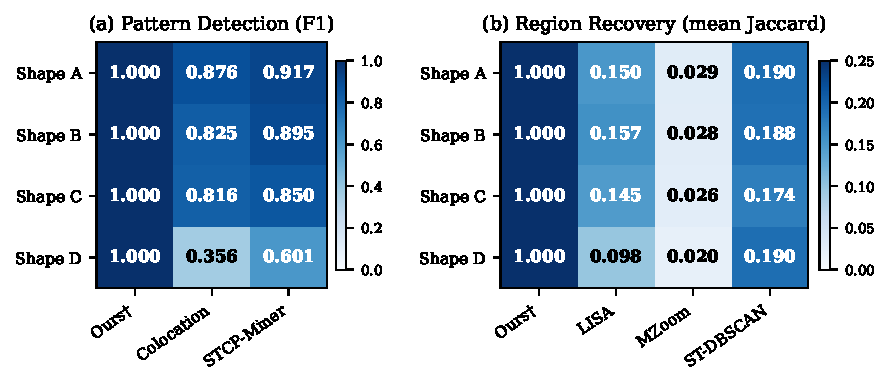
\includegraphics[width=0.90\columnwidth]{fig/fig_ex1_heatmap.pdf}
\caption{EX-1 results (3-seed average, $p_{\mathrm{embed}}{=}0.25$).
  (a)~EX-1-1 F1; (b)~EX-1-2 mean Jaccard.
  GT is the exact solution under the sliding-window definition (Definitions~3--5).
  $\dagger$The proposed method outputs the exact solution by construction,
  hence F1 $= 1.00$ and Jaccard $= 1.00$.
  Baseline parameters were selected by grid search.}
\label{fig:ex1}
\end{figure}

\paragraph{Analysis.}
The proposed method achieves F1\,$=1.00$ and Jaccard\,$=1.00$ by construction,
while existing methods achieve at most F1\,$=0.917$ and Jaccard\,$=0.190$.
---~\textbf{LISA}: collapses occurrences over all time steps, discarding temporal structure.
---~\textbf{MZoom}: Cartesian-product constraint forces convergence to width-1 blocks on a sparse grid.
---~\textbf{ST-DBSCAN}: labels only occurrence cells, missing non-occurrence cells inside dense windows.
These structural mismatches---not parameter tuning---explain
why no baseline approximates the sliding-window definition well across all shapes.

% ==============================================================
\subsection{EX-2: Scalability (Synthetic Data)}
\label{sec:ex2}
% ==============================================================

\paragraph{Objective.}
We evaluate how runtime and peak memory scale
with respect to four parameters independently:
number of temporal grid points $T$,
spatial grid points $S$,
number of dimensions $d$,
and item-set size $|\mathcal{I}|$.

\paragraph{Synthetic data generation.}
On a $d$-dimensional lattice, each item was independently sampled from
Bernoulli$(p_{\mathrm{item}}{=}0.10)$ for all cells to form one basket.
Empty cells were assigned item~1 by default,
ensuring exactly one transaction per cell
(generation details in Appendix~\ref{sec:ex2_data_details}).

\paragraph{Proposed method parameters.}
$W = (24, 4)$ and $\theta = 15$ were fixed throughout.
Base configuration: $T{=}1{,}000$, $S{=}100$, $d{=}2$, $|\mathcal{I}|{=}20$.

\paragraph{Experimental design.}
Four axes are evaluated independently:
(a)~$T \in \{10^2, 10^3, 10^4, 10^5\}$ ($S{=}100$, $d{=}2$);
(b)~$S \in \{10, 10^2, 10^3, 10^4\}$ ($T{=}1{,}000$, $d{=}2$);
(c)~$d \in \{2, 3, 4\}$ with $N{\approx}10^5$ fixed by adjusting spatial dimensions;
(d)~$|\mathcal{I}| \in \{20, 40, 60, 80\}$ ($T{=}1{,}000$, $S{=}100$, $d{=}2$).

\paragraph{Analysis.}
Fig.~\ref{fig:ex2_scalability} shows runtime and peak RSS for all four axes.
Both $T$- and $S$-scalability are approximately linear in $N$:
as $N$ grows from $10^4$ to $10^7$, runtime increases ${\approx}10^3$-fold ($0.046$\,s to $49.5$\,s),
and a higher $T/S$ ratio is slightly faster due to more effective gap-skipping (Lemma~\ref{lem:stride}).
An extended run at $N{=}10^8$ ($T{=}10^6$, $S{=}100$) completes in $517$\,s ($<9$\,min), consistent with linear scaling.
Increasing $d$ from 2 to 4 raises $W_{\mathrm{sp}}$ from 5 to 125 ($25{\times}$),
yet peak memory grows only $1.35\times$, reflecting multiset sparsity per spatial start point.
$|\mathcal{I}|$-scalability is well below exponential,
as Apriori pruning suppresses candidate expansion for non-dense patterns.

\begin{figure}[t]
\centering
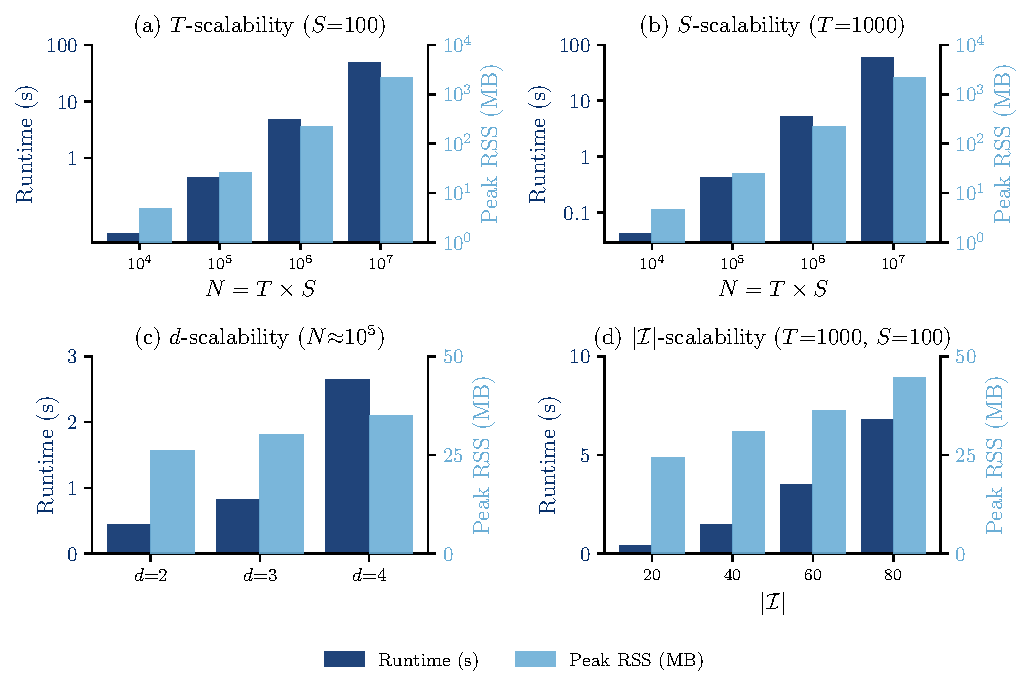
\includegraphics[width=\columnwidth]{fig/fig_ex2_scalability.pdf}
\caption{EX-2: Scalability across four parameters
  ($W{=}(24,4)$, $\theta{=}15$, $p_{\mathrm{item}}{=}0.10$).
  Dark bars: runtime (left axis); light bars: peak RSS memory (right axis).}
\label{fig:ex2_scalability}
\end{figure}

% ==============================================================
\subsection{EX-3: Application to Real-World Data ($d{=}3$--$4$)}
\label{sec:ex3}
% ==============================================================

\paragraph{Objective.}
We applied the proposed method to real-world data from diverse domains
and found that the detected patterns and dense regions
yield interpretable insights consistent with domain knowledge.

\paragraph{Datasets and results.}
Two crime report datasets
(Chicago Crime~\cite{chicagocrime}, NYPD Crime~\cite{nypdcrime}),
citizen complaints (NYC 311~\cite{nyc311}),
and an earthquake catalog (USGS Earthquake~\cite{usgseq})
were used, spanning three domains and $d{=}3$--$4$ dimensions.
Time was discretized into weekly bins and spatial coordinates
into equal-width bins, converting each cell's events into a transaction.
Dataset details and quantitative results
are given in Appendix~\ref{sec:dataset_details}.

\paragraph{Findings.}
Detection counts and runtimes are in Table~\ref{tab:realdata_npatterns} (Appendix~\ref{sec:dataset_details}).
\emph{Chicago Crime} (2,835 patterns):
pairs such as \textsc{Assault}\,+\,\textsc{Battery} form chronic dense windows
in south and west side districts;
three-item patterns (e.g., \textsc{Theft}\,+\,\textsc{Criminal Damage}\,+\,\textsc{Battery})
pinpoint compound hotspots that per-category frequency analysis misses.
\emph{NYPD Crime} (4,478 patterns):
compound co-occurrences of felonies (Felony Assault, Robbery) and
misdemeanors (Petit Larceny, Criminal Mischief)
are captured at borough-and-weekly granularity,
revealing locally concentrated combinations invisible to global frequency rankings.
\emph{NYC~311} (5,130 patterns):
Noise\,--\,Residential and Illegal Parking repeatedly co-concentrate
in residential neighborhoods;
seasonal three-complaint patterns emerge in specific boroughs,
providing week-level actionable signals for policy planning.
\emph{USGS Earthquake} (18 patterns, 4-D):
co-occurrence of M3.0--4.0 and M4.0--5.0 within a depth--time--space window
indicates aftershock sequences;
the depth axis distinguishes shallow crustal events (${\lesssim}30$\,km)
from intermediate-depth intraslab events,
consistent with subduction-zone structure.
In all cases the method outputs \emph{which} itemsets are dense and
\emph{when and where} as concrete windows,
providing interpretable results for domain experts.

% ==============================================================
\section{Conclusion}\label{sec:conclusion}
% ==============================================================

This paper proposed \textbf{Multi-Dimensional Apriori-Window},
which extends Apriori-Window~\cite{aprioriwindow}
to arbitrary $d$-dimensional grids.
Through three techniques---one-dimensional multiset reduction
per fixed spatial start point,
duplicate-aware $t$-axis stride,
and $(k{-}1)$-subset interval map intersection pruning---the method
exactly enumerates all dense patterns
together with their arbitrarily-shaped dense regions.

Experiments demonstrated that:
(1)~on synthetic data with four embedding shapes,
the proposed method outputs the exact solution,
while existing methods achieved at most
F1\,$=0.917$ and Jaccard\,$=0.190$;
(2)~the proposed method demonstrated linear scaling
for $N = 10^4$--$10^8$,
processing $10^8$ transactions within 9 minutes;
(3)~on $d{=}3$--$4$ real-world data from crime, complaints,
and earthquake domains,
the method yielded interpretable insights
consistent with domain knowledge,
such as compound crime hotspots
and depth-stratified seismic clusters.

\paragraph{Limitations.}
\begin{itemize}
    \item \textbf{Grid discretization:} Results depend on the choice of bin width and $\bm{W}$.
    \item \textbf{Scalability in high dimensions:} Multiset construction costs $O(N \cdot W_{\mathrm{sp}})$, which becomes expensive as $d$ or $W_{\mathrm{sp}}$ increases.
    \item \textbf{No causal explanation:} The method detects and describes dense patterns and regions, but does not explain their causes or associations with external events.
\end{itemize}

\paragraph{Future work.}
\begin{itemize}
    \item \textbf{Adaptive parameter selection:} Automatically determine $\bm{W}$ and $\theta$ from local data statistics, such as density distributions and spatial autocorrelation.
    \item \textbf{Further acceleration:} Reduce redundant multiset construction using prefix-sum-based $O(1)$ window aggregation and incremental updates along spatial axes.
\end{itemize}


% --- Acknowledgment ---
\section*{Acknowledgments}
This work is supported by the Honda Bridge Project.
The authors also acknowledge that portions of the text in
this paper were generated with Anthropic's large language
model Claude~\cite{claude2025}.

% --- References ---
\newpage
\bibliographystyle{IEEEtran}
\bibliography{refs}

% --- Appendix ---
\clearpage
\appendices
% ==============================================================
\section{Complexity Analysis}
\label{sec:complexity_appendix}
% ==============================================================

\begin{table}[h]
\centering
\caption{Computational complexity of the proposed method.
$N_P$: number of transactions containing pattern $P$,
$W_{\mathrm{sp}} = \prod_{k=1}^{d-1} (W_k + 1)$,
$\widetilde N_P = N_P W_{\mathrm{sp}}$,
$I_P$: total number of intervals in the candidate interval map.}
\label{tab:complexity}
\small
\begin{tabular}{lll}
\toprule
Step & Complexity \\
\midrule
Construction of $L_P$ & $O(N_P \cdot W_{\mathrm{sp}})$ \\
Sorting of $L_P$ & $O(\widetilde N_P \log \widetilde N_P)$ \\
Temporal interval & \multirow{2}{*}{$O\!\left(\sum_{\bm{s}_{\mathrm{sp}}}|L_P(\bm{s}_{\mathrm{sp}})| \log |L_P(\bm{s}_{\mathrm{sp}})|\right)$} \\
\quad computation & \\
Candidate interval & \multirow{2}{*}{$O(I_P)$} \\
\quad map intersection & \\
\bottomrule
\end{tabular}
\end{table}

The overall complexity faithful to the current implementation is
\[
  O\!\left(
    \sum_{P \in \mathcal{F}}
      \bigl(
        N_P W_{\mathrm{sp}}
        +
        \widetilde N_P \log \widetilde N_P
        +
        I_P
      \bigr)
  \right)
\]
where $\mathcal{F}$ is the set of candidate patterns actually evaluated.
The key factor governing practical complexity is $|\mathcal{F}|$,
which is controlled by Apriori pruning (Lemma~\ref{lem:apriori}):
any pattern whose $(k{-}1)$-subsets have empty candidate interval maps is pruned
without evaluation, bounding $|\mathcal{F}|$ to the set of dense patterns.
In the worst case, when all itemsets are dense,
$|\mathcal{F}|$ grows exponentially in $|\mathcal{I}|$;
this is inherent to any exact enumeration algorithm and is
mitigated in practice by the sparsity of real transaction data.

% ==============================================================
\section{Proofs of Lemmas}
\label{sec:proofs}
% ==============================================================

\begin{proof}[Proof of Lemma~\ref{lem:apriori}]
For any transaction $n$, if $P \subseteq d_n$ then $Q \subseteq d_n$.
Therefore, for any fixed spatial start vector $\bm{s}_{\mathrm{sp}}$,
each element of $L_P(\bm{s}_{\mathrm{sp}})$
is also contained in $L_Q(\bm{s}_{\mathrm{sp}})$.
Hence, for any $s_0$,
$S_P(s_0,\bm{s}_{\mathrm{sp}}) \leq S_Q(s_0,\bm{s}_{\mathrm{sp}})$ holds.
\end{proof}

\begin{proof}[Proof of Lemma~\ref{lem:stride}]
Consider the rightmost $\theta$ events within the current window
$[l, l+W_0]$.
The leftmost of these is $L[l_{\mathrm{lo}} + (c-\theta)] = l_{\mathrm{dense}}$.
For any $l' \leq l_{\mathrm{dense}}$,
all $\theta$ events are $\geq l'$,
and since $l' \geq l$, we have $l'+W_0 \geq l+W_0$.
Therefore, these events do not leave the current window $[l,l+W_0]$
and are all contained in $[l', l'+W_0]$ as well.
Hence, at least $\theta$ events remain within the window at $l'$.
\end{proof}


% ==============================================================
\section{EX-1 Synthetic Data Generation Details}
\label{sec:ex1_data_details}
% ==============================================================

\paragraph{Background data generation.}
One transaction is placed at every grid point of a
$T{=}100 \times S{=}100$ grid.
With $|\mathcal{I}|{=}40$ items,
each item is independently sampled from
Bernoulli$(p_{\mathrm{item}}{=}0.15)$ per cell to form the background.
Cells where all items are absent are assigned item~1 by default.

\paragraph{Pattern embedding.}
GT patterns $P_k = \{2k{-}1,\, 2k\}$ ($k=1,\ldots,20$)
are assigned to spatial bands
$s \in [5(k{-}1),\; 5(k{-}1){+}4]$ (width 5 cells).
Within cells belonging to the embedding region of each shape,
item pair $P_k$ is co-embedded independently with
Bernoulli$(p_{\mathrm{embed}}{=}0.25)$.

\paragraph{Embedding shapes.}
Each shape specifies the spatio-temporal distribution of pattern $P_k$
within its spatial band
($b_s = 5(k-1)$, $b_e = b_s + 4$).

\begin{itemize}
\item \textbf{Shape A (rectangular)}:
  Uniformly embedded in all cells with
  $t \in [30,70]$ and $s \in [b_s, b_e]$.
  The simplest fixed rectangular region in both time and space.
\item \textbf{Shape B (drift)}:
  At each time step $t \in [30,70]$,
  a band of width 5 is centered at
  $s_c = \lfloor b_s + (t - 30) / 40 \cdot 2 \rceil$
  (linearly shifting from $b_s$ to $b_s{+}2$).
  The dense band drifts smoothly along the spatial axis over time.
\item \textbf{Shape C (intermittent)}:
  $t \in [15,35] \cup [65,85]$, $s \in [b_s, b_e]$.
  Dense activity occurs in the same spatial band
  during two independent time intervals.
\item \textbf{Shape D (expanding)}:
  $t \in [30,40]$: center cell $b_s{+}2$ only (width 1);
  $t \in [41,55]$: $s \in [b_s{+}1, b_e{-}1]$ (width 3);
  $t \in [56,70]$: $s \in [b_s, b_e]$ (width 5).
  The spatial extent grows stepwise as time progresses.
\end{itemize}

\paragraph{Evaluation setup.}
Three random seeds (seed $\in \{42,55,68\}$) are used per shape,
giving $4 \times 3 = 12$ datasets in total.
The proposed method uses $W = (20, 5)$ and $\theta = 30$
uniformly across all shapes.
Grid search parameter ranges are shown in Table~\ref{tab:params_ex3}.

\begin{table}[h]
\centering
\caption{Grid search parameter ranges for EX-1 baseline methods.}
\label{tab:params_ex3}
\small
\begin{tabular}{lp{0.62\columnwidth}}
\toprule
Method & Grid search targets \\
\midrule
Colocation   & PI threshold $\tau \in \{0.05, 0.07, \ldots, 0.49\}$ (23 values) \\
STCP-Miner   & PI threshold (same) $\times$ window width $W_t \in \{4, 13, 26, 54\}$ \\
MZoom        & Top block count $k \in \{1, 2, 3, 5\}$ \\
ST-DBSCAN    & $\varepsilon_1 \in \{1,2,3\}$, $\varepsilon_2 \in \{3,7,15\}$, min\_pts $\in \{2,5\}$ \\
\bottomrule
\end{tabular}
\end{table}

% ==============================================================
\section{EX-2 Synthetic Data Generation Details}
\label{sec:ex2_data_details}
% ==============================================================

In EX-2, synthetic data is generated by placing
one transaction at \textbf{every} grid point of a $d = 2$ grid
$\{0,\ldots,T{-}1\} \times \{0,\ldots,S{-}1\}$.
For each transaction,
each item is independently sampled from
Bernoulli$(p_{\mathrm{item}})$ with
vocabulary size $|\mathcal{I}| = 20$ and
background occurrence probability $p_{\mathrm{item}} = 0.10$.
Cells where all items are absent
are assigned item~1 by default,
guaranteeing exactly one transaction per cell.
This ensures the number of transactions is exactly $N = T \times S$.

No embedded patterns are injected.
Dense patterns arise naturally from
statistical fluctuations of the Bernoulli background.
Preliminary calibration showed that
a sufficient number of patterns is detected
at threshold $\theta = 15$ across all configurations.


% ==============================================================
\section{Real Dataset Details}
\label{sec:real_data_qualitative}\label{sec:dataset_details}
% ==============================================================

\paragraph{Dataset overview.}
The four real-world datasets used in EX-3 (\S\ref{sec:ex3}) are detailed below.

\begin{itemize}
\item \textbf{Chicago Crime}~\cite{chicagocrime}:
  Crime report data published by the City of Chicago.
  Includes date/time, latitude, longitude,
  and crime type (33 types).
  Time discretized into weekly bins;
  latitude and longitude into $0.02^\circ$ equal-width bins
  (grid size $261 \times 20 \times 21$).
\item \textbf{NYPD Crime}~\cite{nypdcrime}:
  Crime report data published by the New York City Police Department.
  Includes crime type (69 types).
  Weekly bins, $0.02^\circ$ spatial bins
  (grid size $261 \times 43 \times 57$).
\item \textbf{NYC 311}~\cite{nyc311}:
  Citizen complaint (311) data from New York City.
  Includes complaint type (232 types).
  Weekly bins, $0.02^\circ$ spatial bins
  (grid size $261 \times 43 \times 57$).
\item \textbf{USGS Earthquake}~\cite{usgseq}:
  Earthquake catalog published by the United States Geological Survey.
  Magnitude discretized into 5 bands and used as items.
  This is the only 4-dimensional dataset
  (time $\times$ latitude $\times$ longitude $\times$ depth),
  with grid size $1{,}096 \times 20 \times 20 \times 4$.
\end{itemize}

\begin{table}[h]
\centering
\caption{Experimental datasets.
$N$: number of transactions (non-empty cells),
\#Items: number of item types,
avg$\ell$: average items per transaction,
$d$: dimensionality.}
\label{tab:datasets}
\small
\begin{tabular}{lrrrr}
\toprule
Dataset & $N$ & \#Items & avg$\ell$ & $d$ \\
\midrule
Chicago Crime~\cite{chicagocrime}  &  47,217 &  33 &  7.59 & 3 \\
NYPD Crime~\cite{nypdcrime}        & 189,481 &  69 &  5.67 & 3 \\
NYC 311~\cite{nyc311}              & 135,490 & 232 & 18.14 & 3 \\
USGS Earthquake~\cite{usgseq}      &  13,151 &   5 &  1.17 & 4 \\
\bottomrule
\end{tabular}
\end{table}

\paragraph{Experimental parameters.}
Maximum pattern length $|P| \leq 3$ was used for all datasets.
The three 3-dimensional datasets (Chicago/NYPD/NYC~311) share
temporal window $W_0 = 4$ weeks and spatial windows $W_k = 3$ bins
($k = 1, 2$), with only threshold $\theta$ adjusted per dataset.
USGS Earthquake used $W_0 = 13$ weeks, $W_k = 2$ bins ($k = 1,2,3$),
and $\theta = 2$.

\begin{table}[h]
\centering
\caption{Detection results of the proposed method on real datasets.
  $\theta$: density threshold,
  Total: number of patterns (all sizes),
  time: execution time (seconds).}
\label{tab:realdata_npatterns}
\small
\begin{tabular}{lrrrr}
\toprule
Dataset & $W$ & $\theta$ & Total & time (s) \\
\midrule
Chicago Crime  & $(4,3,3)$    &   3 & 2,835 &   9.7 \\
NYPD Crime     & $(4,3,3)$    &   5 & 4,478 &  38.2 \\
NYC 311        & $(4,3,3)$    &  35 & 5,130 & 108.7 \\
USGS Earthq.   & $(13,2,2,2)$ &   2 &    18 &   0.5 \\
\bottomrule
\end{tabular}
\end{table}


\end{document}
